\tikzset{every picture/.style={line width=0.75pt}} %set default line width to 0.75pt        

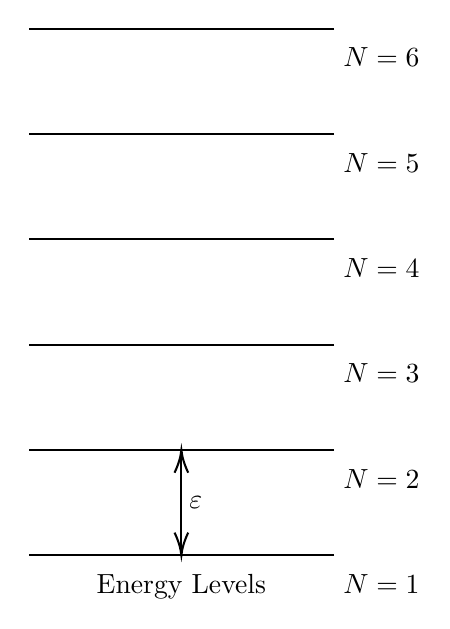
\begin{tikzpicture}[x=0.75pt,y=0.75pt,yscale=-1,xscale=1]
%uncomment if require: \path (0,321); %set diagram left start at 0, and has height of 321

%Straight Lines [id:da9794122444476456] 
\draw    (397.39,257.47) -- (250.29,257.47) ;
%Straight Lines [id:da22687544885274602] 
\draw    (397.39,206.73) -- (250.29,206.73) ;
%Straight Lines [id:da28467543369498616] 
\draw    (397.39,155.99) -- (250.29,155.99) ;
%Straight Lines [id:da32926947196763545] 
\draw    (397.39,105.25) -- (250.29,105.25) ;
%Straight Lines [id:da4596445103814899] 
\draw    (397.39,54.5) -- (250.29,54.5) ;
%Straight Lines [id:da5432766471171577] 
\draw    (397.39,3.76) -- (250.29,3.76) ;
%Straight Lines [id:da8263951695821707] 
\draw    (323.84,208.73) -- (323.84,255.47) ;
\draw [shift={(323.84,257.47)}, rotate = 270] [color={rgb, 255:red, 0; green, 0; blue, 0 }  ][line width=0.75]    (10.93,-3.29) .. controls (6.95,-1.4) and (3.31,-0.3) .. (0,0) .. controls (3.31,0.3) and (6.95,1.4) .. (10.93,3.29)   ;
\draw [shift={(323.84,206.73)}, rotate = 90] [color={rgb, 255:red, 0; green, 0; blue, 0 }  ][line width=0.75]    (10.93,-3.29) .. controls (6.95,-1.4) and (3.31,-0.3) .. (0,0) .. controls (3.31,0.3) and (6.95,1.4) .. (10.93,3.29)   ;

% Text Node
\draw (400.38,265.19) node [anchor=north west][inner sep=0.75pt]   [align=left] {$\displaystyle N=1$};
% Text Node
\draw (400.38,214.45) node [anchor=north west][inner sep=0.75pt]   [align=left] {$\displaystyle N=2$};
% Text Node
\draw (400.38,163.71) node [anchor=north west][inner sep=0.75pt]   [align=left] {$\displaystyle N=3$};
% Text Node
\draw (400.38,112.96) node [anchor=north west][inner sep=0.75pt]   [align=left] {$\displaystyle N=4$};
% Text Node
\draw (400.38,62.22) node [anchor=north west][inner sep=0.75pt]   [align=left] {$\displaystyle N=5$};
% Text Node
\draw (400.38,11.48) node [anchor=north west][inner sep=0.75pt]   [align=left] {$\displaystyle N=6$};
% Text Node
\draw (326.14,232.1) node [anchor=west] [inner sep=0.75pt]   [align=left] {$\displaystyle \varepsilon $};
% Text Node
\draw (323.84,264.99) node [anchor=north] [inner sep=0.75pt]   [align=left] {Energy Levels};


\end{tikzpicture}
